\title{Proposed - Parameter Optimization Method for Dynamically Controlled Optical Systems Via Kinetic Time-domain Simulation}

% typeset with pdflatex, bibtex, pdflatex, pdflatex

\documentclass{aiaa-tc}

 \author{Timothy E. Coon%
         \thanks{PhD Student, MAE}\\
         \normalsize\itshape
         FIT, Melbourne, Florida, 32901, USA}

\begin{document}

\maketitle

\begin{abstract}
This paper introduces the theory of proposed research. The research goal is to develop a methodology and associated techniques by which to close the outermost loop on the optomechanical design process of a space-based optical system with dynamic controllers for disturbance rejection. The outermost design loop considers the effect of static system design parameters on a dynamic cost function over a finite time of operational disturbance rejection. Currently, several design loops are integrated throughout the static and quasi-static design process of an optical system and these are discussed briefly. This research considers the effect of real-time kinetics on an appropriate cost functional insofar as it may influence static parameter design decisions for optical prescription (e.g. focal length).
\end{abstract}

% \section*{Nomenclature}
%
% \begin{tabbing}
%   xxxxx \= \kill % first line sets tab stop
%   $J$ \> Jacobian Matrix \\
%   $f$ \> Residual value vector \\
%   $x$ \> Variable value vector \\
%   $F$ \> Force, N \\
%   $m$ \> Mass, kg \\
%   $T$ \> Test \\
%   $\Delta x$ \> Variable displacement vector \\
%   $\alpha$ \> Acceleration, m/s\textsuperscript{2} \\[5pt]
%   \textit{Subscript}\\
%   $i$ \> Variable number \\
%   $i$ \> Variable number \\
%  \end{tabbing}

\section{Introduction}

This paper is written to introduce interested parties to proposed research. It is intended as a starting point for soliciting feedback on the advantage and originality successful completion of the research offers. The proposed research focuses on space-based optical system design.

\subsection{Background}

Optomechanical design processes to date implement a number of design iteration loops, some abstract and others methodical. There are a number of useful software-based design and simulation tools utilized in various combinations and with techniques specific to industries and individual organizations.

\begin{figure}[htb]	% YingDesignProcess
 \centering
 \includegraphics[width=0.75\textwidth]{Figures/Yingling_IntegratedDesignProcess}
 \caption{The integrated Design process for a segmented mirror system (Yingling)}
 \label{YingDesignProcess}
\end{figure}

Reference Figure~\ref{YingDesignProcess} illustrating the design process for the Segmented Mirror Telescope testbed at The Naval Postgraduate School, Figure~\ref{SMT}. The integration of systems engineering, optics, structures, and controls on the path to a finished optical system is a complex mechanism, each aspect having design criteria in conflict with those of other disciplines. Several design iteration loops are recognizable within this illustration. Following the implementation of traditional design loops illustrated, a robust optical system design is established with mitigation of operational environment impact on image quality. A control law is then applied to the system to correct for environmental disturbances. (Burl, Yingling, Redding, etc). An optimal control law maximizes the sytem performance either in practice with real-time linear/nonlinear robust control (Burl, Slotine/Li) or theoretically using a-priori disturbance and optimization methods (i.e. LGR collocation \& NLP). It is at this point the improvement efforts have concluded in previous work.

\begin{figure}[htb]	% SMT
 \centering
 \includegraphics[width=0.5\textwidth]{Figures/SMT}
 \caption{The Segmented Mirror Telescope (Yingling)}
 \label{SMT}
\end{figure}

% After defining subsytem requirements, the next task is to design the optical system and build simulations using software packages such as Zemax's Optic Studio\textsuperscript{\texttrademark}. Zemax allows for some quasi-static optimization methods based on user-defined merit functions. This analysis allows the designer to minimize optical performance sensitivities such as those impacted by imperfections in realized hardware. After having established an optical prescription with optical elements located in three-dimensional space, the designer uses CAD tools to design the structure locating the surface elements precisely where the optical model prescribes. During this stage, conflicts may arise between the necessary structure and the desired optical prescription requiring changes to the original optical prescription. After a mechanical design is established the mode shapes of the structure are found using finite element analysis software. These mode shapes may then be applied to the optical model to determine the optical performance sensitivity to deflection of each significant mode shape. These structural mode shapes are then used to simulate misalignments in the optical system and the optical simulation software is used to change the optical prescription to mitigate image degradation as a result of misalignment caused by the mode shape deflection. The final design loop currently implemented is:

% \begin{tabbing}
% Design Loop \#1: Mission Requirements $\leftrightarrow$ Zemax \\
% Design Loop \#2: Zemax $\leftrightarrow$ CAD (Static) \\
% Design Loop \#3: Zemax $\leftrightarrow$ CAD (Mode Shape Deflections) \\
% Design Loop \#4: Actuator performance $\leftrightarrow$ CAD $\leftrightarrow$ Zemax \\
% Proposed Design Loop: End-End Dynamically Controlled System $\leftrightarrow$ Zemax $\leftrightarrow$ CAD
% \end{tabbing}

\section{Proposed Research}

The goal of the proposed research is the formalization of methods and techniques for optimal optical-system design given limits on the operational environment. More specifically, the development of the design loop shown in red on Figure~\ref{YingDesignProcess} which iterates on the optical design using dynamic controller performance metrics. This idea is presented more thoroughly by example.

% \section{Random Noise}
%
% At this stage, the noise comprises sine wave inputs at specified frequencies (resonant frequencies). The magnitude of the sine waves are constant as they would likely be for short camera integration times. The randomness of the input is entirely in the phase shift of the input sine waves.

\section{Linear Feedback Example}

A simple example is presented showing the impact of optical parameter selection in dynamic operation of a telescope. Figure~\ref{simplefig} shows a collimated input beam entering from the top, parallel to the principal axis of a parabolic mirror. It strikes the parabolic mirror surface off-axis and is reflected to a reference surface at the origin. The arrows show the path and direction of the rays, the `+' symbols are the ray-surface intersection points and the dots are the vertices of the surfaces.



Figure~\ref{KinSys} shows the dynamic system operation with white noise input disturbance torque and control torque generated by PD-feedback controller. Both the input disturbance and the control torque are applied at a point just behind the intersection of the chief ray with the parabolic mirror. The control is applied to reduce the angular pointing error of the parabolic mirror. Due to the inability of the dynamic controller to perfectly correct for the input disturbance, there will be some degradation of the image as seen at the reference surface. This degradation is quantified using rms spot size. It is determined this system should have field of view and magnification limits given by focal lengths between $f_{min} = 0.70 m$ and $f_{max} = 0.80 m$. It is assumed magnification is more desirable so a cost is associated with focal lengths away from $f_{min}$. The total cost is then a combination of rms spot size and focal length. Figure~\ref{costPlots} shows the control vector, instantaneous cost, and running cost vs time. The running cost is merely the scaled rms spot size integrated over time plus the focal length deviation cost.


The cost plots reveal the dependence of dynamic performance on the focal length of the system. The vertical line shows the time when the minimum cost switches from one focal length to the other. If we consider a finite camera integration time, the image quality can be linked directly to the running cost. For this disturbance profile and this particular cost function, the shorter focal length yields better performance for integration times greater than about 0.13 seconds, see Figure~\ref{zoomCost}.
\bigskip

\section{Conclusion}

The illustration of this simulation demonstrates the dependence of parameter selection on the system performance in the dynamic environment. Furthermore, generalizations are difficult to make. Unlike in frequency anlysis, it is not possible to characterize a design parameter as ``better" given established values such as system natural frequency. Instead, we must consider the performance of a system design for a specified input disturbance using fuzzy cost functionals. Conclusions are drawn from distinct input disturbances, so it is necessary to establish stochastic definition of the input disturbances and transform this to a statistical measure of output performance. This is done by implementing Monte Carlo or Polynomial Chaos methods. An example of this input-statistics-to-output-statistics for an open-loop system will be presented at a later date.

\section{Big Picture}
The end goal is a methodology to optimize the design of a dynamically controlled optical system operating in a known environment. The steps are listed below.

\begin{enumerate}
	\item Define input disturbances stochastically.
	\item Specify dynamically controlled optical system with $n$ design parameters.
	\item Generate a realization of the stochastic input disturbance and calculate the output performance with the optimal control solution.
	\item Repeat 3 with enough realizations to generate statistics for the output performance.
	\item Repeat 2-4 using new set of $n$ design parameters.
	\item Optimize $n$ design parameters to yield the optimal output performance distribution (e.g. reduce mean of crossover time for the example above). A brute-force approach to this end is computationally improbable so advanced numerics and optimizaiton algorithms will need to be researched, enhanced, and applied.
\end{enumerate}

Note: I choose to use an optimal control solution because it is the limit of best performance and isn't sensitive to changing design parameters. I am able to do this because I know the disturbance a priori for each realization. Real-time controllers may operate with better performance for a different design point and this will be a question addressed in the research.

Elements of this research are summarized in the table below.

\begin{table}
  \centering
  \caption{Research Elements}
  \label{t:researchElements}
  \begin{tabular}{cc}
       \# & Element \\\hline
        1 &  Optical system design and simulation (linear \& nonlinear) \\
        2 &  Control system design and simulation (linear \& nonlinear) \\
        3 &  Environment noise uncertainty models \\
        4 &  Dynamic optimal control \\
        5 &  Finite element analysis 
  \end{tabular}
\end{table}
\
More information to follow!!

\newpage


\begin{figure}[t]	% simplefig
 \centering
 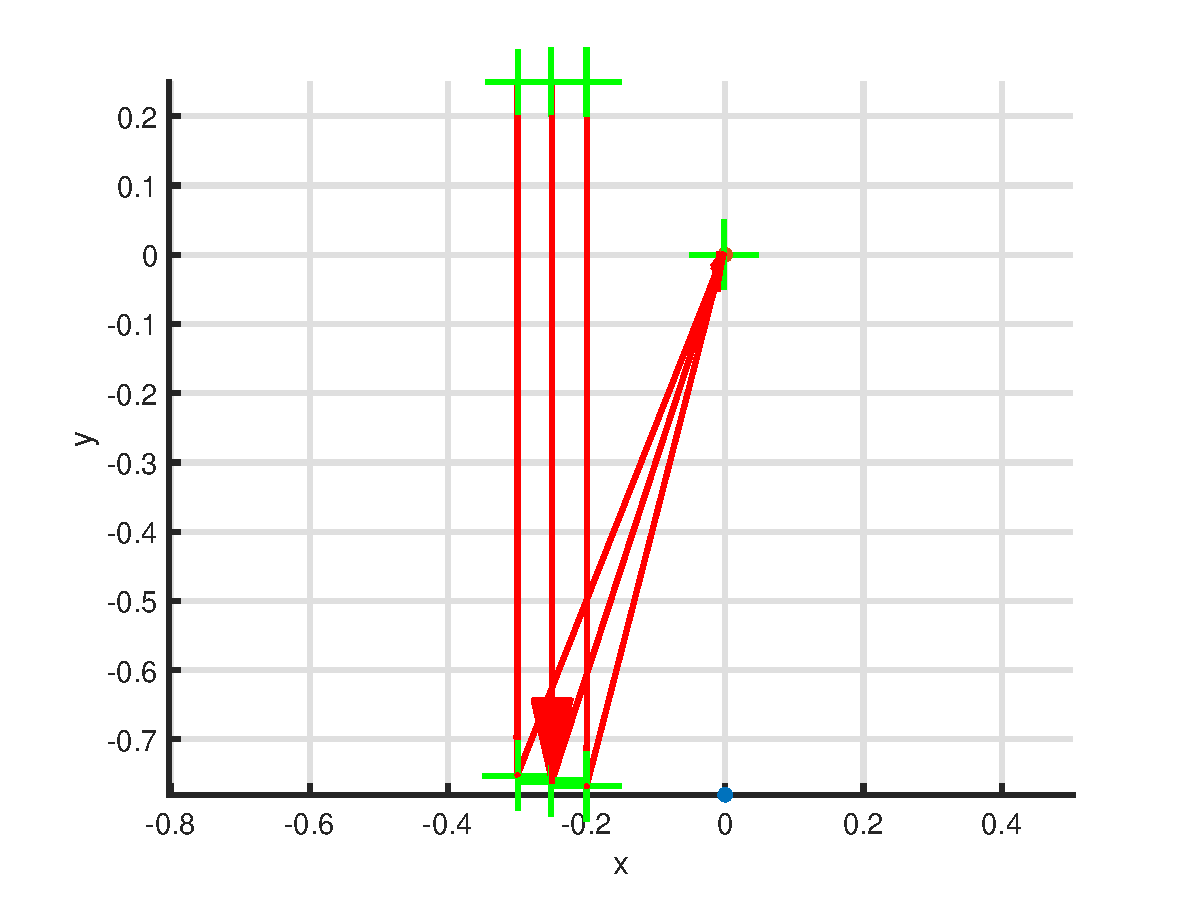
\includegraphics[height=0.5\textwidth,trim={2cm 0 0 1cm}]{Figures/SimpleLayout}
 \caption{Simple System Layout}
 \label{simplefig}
\end{figure}

\begin{figure}[b]	% KinSys
 \centering
 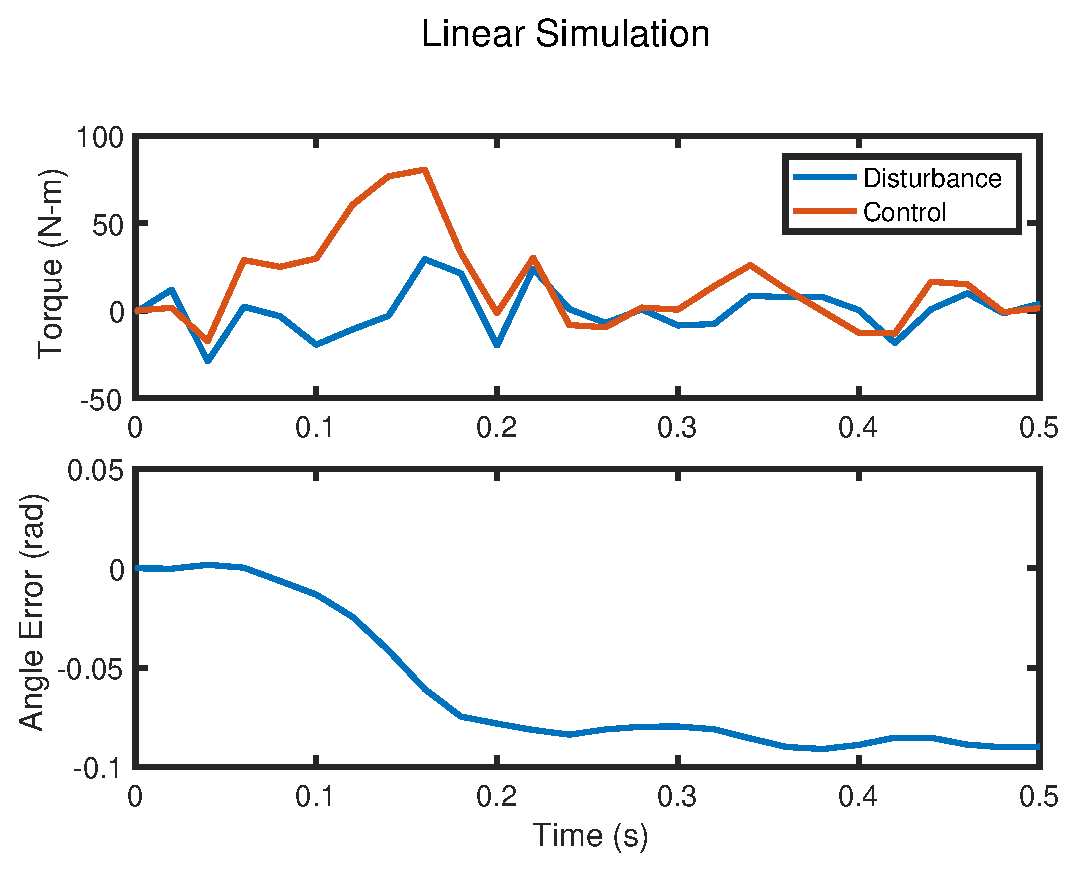
\includegraphics[height=0.5\textwidth,trim={2cm 0 0 1cm}]{Figures/dynamicsPlot}
 \caption{Kinetic System Control}
 \label{KinSys}
\end{figure}

\begin{figure}[t]	% costPlots
 \centering
 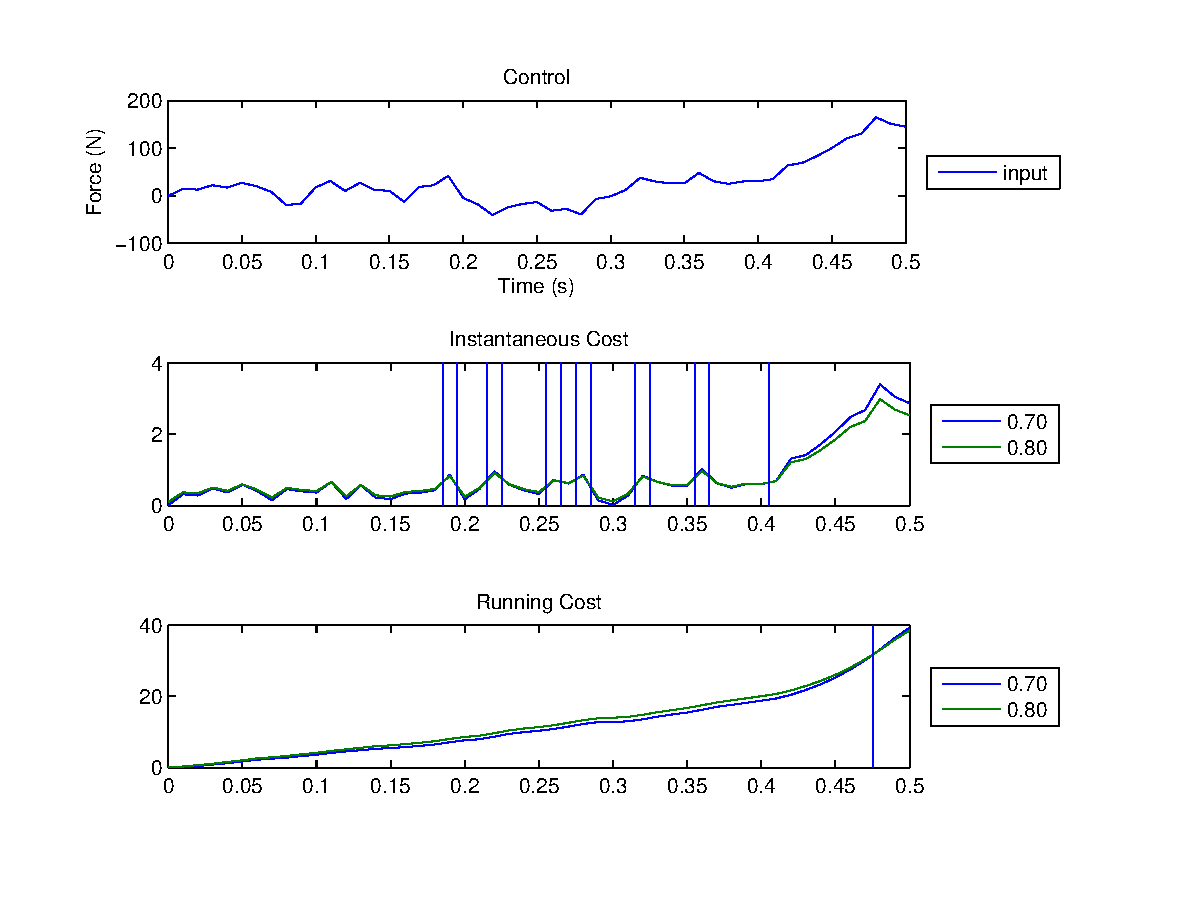
\includegraphics[height=0.5\textwidth]{Figures/costPlots}
 \caption{Control and cost plots.}
 \label{costPlots}
\end{figure}

\begin{figure}[b]	% zoomCost
 \centering
 \includegraphics[height=0.5\textwidth]{Figures/zoomCostPlot}
 \caption{Zoom in to see crossover point.}
 \label{zoomCost}
\end{figure}

% The longer focal length accrues less cost when the control input is greater for the range considered here. At first glance, this seems counterintuitive because a longer focal length is more susceptible to being off-target given a specified angular error. However, notice the solid angle of the beam at the focal point is smaller for a longer focal length. This means an angular error results in less enlargement of the rms spot radius for a longer focal length and rms spot radius is the only image quality cost. If deviation of the chief ray were also a considered cost, then the results may be different.
%
% Assume I know the integration time of my camera is 0.3 seconds. At this time, for the presented simulation, the shorter focal length yields better performance for this time. If we open the design space to include any focal length in the range, then we will likely find a focal length between $f_max$ and$f_min$ to yield better performance. The focus of this research is the method by which to determine this optimal design parameter, or, in general, the set of optimal design parameters for an optical system.
%
% Effectively, the dynamic optimization proposed here is an enhancement on the design loop considering the optical sensitivities to misalignments in the optical system. Whereas, before, the sensitivities may be calculated with the optical prescription perturbed according to the significant mode shapes, a stochastic dynamic control estimate allows the designer to evaluate the degree to which nominal optical performance should be sacrificed to reduce sensitivities based on the ability of control actuators operating in response to the simulated environment.
%
% When you optimize an optical prescription by reducing the sensitivity of optical performance to mode shape deflections, the nominal optical performance is degraded. I am not sure how this process is carried out, but \textbf{I don't see any way of determining the trade-off between mitigating sensitivities and sacrificing nominal performance without some characterization of the dynamic operation in the time domain. Effectively, this is saying a frequency analysis is not adequate for determining the adjustment to the optical prescription.}
%
% It doesn't matter how much you try to move or damp out the natural frequencies, the controller is never able to completely reject a random disturbance input. The response lag time and actuator dynamics keep the system from performing perfectly.
%
% Frequency-domain analysis does not allow the engineer to account for time or for absolute magnitude. Time-domain analysis does not allow the engineer to account for the scope of inputs and outputs possible.

% \section*{Appendix}
%
% An appendix, if needed, should appear before the acknowledgments.
% Use the 'starred' version of the \verb|\section| commands to avoid
% section numbering.
%
% \section*{Acknowledgments}
%
% A place to recognize others or simply thank Kleb and Wood for this template.
%
% \bibliographystyle{aiaa}
% \bibliography{references}

\end{document}